\chapter{Introduction}


\chapterintro*


some text about this chapter~\cite{INTROSAMPLE}

\section{Industrial Revolutions}
Major advances in manufacturing of goods for the betterment of humanity have occurred many times in the last two hundred and fifty years in the history of humanity.  These advancements occurred of science and technology occurred as revolutionary events at different times.  The first revolution occurred at the edge of the eightieth century primarily in England but also in France, Germany, and the United States with the applicant of automatic mechanization of large machines using coal powered steam engines.  These machines were mainly used for the processing of cotton, wool, and silks in the production of textiles for export throughout the world.  Advancements during this period included uses of coal to produce steam power, the production of iron, steel, and other rudimentary alloys, and, very importantly, the engineering advancements of tool making.  The advancements of the first industrial revolution paved the way for the centralization and mass production of goods.
%CITATION SOURCES *** {https://en.wikipedia.org/wiki/Technological_revolution#Potential_future_technological_revolutions}

The next century was marked by the development of scientific and engineering advancements in chemistry, physics, and engineering. Experimentation with electricity and the production thereof led to the eventual explosion of industrial machinery, tooling, electrification, chemical manufacture, petroleum refinement, rail and marine transportation, the automobile, agriculture, and telecommunications by wire over long distances.  This period of discovery culminated with rapid expansion of industrialization through the world, especially in North America and Japan up until the beginning of World War I.
%CITATION SOURCES *** https://en.wikipedia.org/wiki/Second_Industrial_Revolution#Machine_tools

The third industrial revolution began in the tears immediately following the second world war with the rapid advancement of pure and applied sciences.  These advancements were driven primarily by the cold war and the space race between the United States and the USSR.  This period of advancement was marked by many discoveries and scientific applications such as the development of telecommunications theories (Claude Shannon), advancement of radio and wired communications, the discovery of the transistor, and the rapid expansion of computers and information technology in business and defense.  Also during these years, arrived the application of computing within manufacturing and process control settings. Computers slowly began to replace the basic relay circuit in control systems.  By utilizing the programmable logic controller (PLC), manufacturers gained the ability to develop control their processes more easily and develop control strategies that were once more difficult to implement in the past with dedicated, specialized equipment.  PLCs offered both the ability to more easily adapt processes to information gathered directly from the factory operation as well as slowly collect and store information electronically.  However, electronic storage of this information was still both difficult and expensive as telecommunications technology was yet relatively slow and storage expensive.  Over the years following through the 1980's until today, computers have followed closely Moore's "Law" which states according to the the perception of Intel Corporation founder, Gordon E. Moore, that the number of transistors on a microchip doubles every two years.  This paradigm of exponential growth in digital computing technology in terms of computing speed, storage, and efficiency has created a world in which computers and computing devices have become ubiquitous, surrounding practically every aspect of human endeavours and leading to the latest installment of industrial advancement, the 4\textsuperscript{th} Industrial Revolution, also known as the \textit{Information Revolution} which is currently ongoing. 

The Information Revolution is defined by a culture that is highly interconnected and data depended.  Clearly, the modern world is dominated by the Internet, high-performance computers, and personal mobile communications devices such as cell phones developed over the last several decades. Within the hands of each individual one may find a smartphone capable of performing computing and communications tasks not even imaginable fifty years ago.  Indeed, within each of these devices resides a powerful microprocessor capable of clocking speeds in the gigahertz, offline storage spanning gigabytes, at-least one high-resolution camera, and communication components enabling high-speed connectivity capable.  These personal devices are smart and easily re-programmable by downloading of new applications, i.e., \textit{apps} enabling users to produce and consume information rapidly.  Users enjoy the ability to speak at any moment, send brief messages using apps such as WhatsApp\texttrademark, download videos, play games, store documents, music, photographs, and videos within "the cloud."  Within office and business enterprises, a personal computer is within reach of every employee and is the tool used for information production.  The data produced is stored within the cloud and usually produced and maintained locally, although the services of data production are quickly shifting to the cloud as well depending on the needs the end user.

These capabilities have also been permeating industrial environments although at a slower rate given the inherent conservatism of industrial establishments.  Industrial environments include aerospace and automotive manufacturing, electrical power production, food processing, petroleum and chemical production.  That is not to say that industrial establishments are not open to technological change, but that established production system can be difficult or risky to modify once they are operational.  While industrial operations have distinctly different requirements than office businesses; analogues may be made between the computing constructs found within the personal/business computing domains and those constructs founds within the industrial computing domains.  For example, within a factory production enterprise, the Internet itself exists as an outside entity providing global connectivity, hosting, storage, computing resource, and analysis tools.  These services are often replicated within the business enterprise of the factory operation and extended into the factory environment to some degree from the factory management system to the factory floor.  

In addition, with the explosiveness of ubiquitous, low-cost computing devices, the modern factory operation is changing to include more intelligence and adaptability at the factory edge.  This includes discrete devices such as sensors and actuators, collaborative robots, autonomous gantry systems, intelligent vehicular systems, tracking and inventory systems, and the like.  These systems coupled with the plethora of computing resources have the potential to create an enormous amount of information as well as the opportunities for greater control over the factory enterprise.  It is just a matter of tapping the information within the factory and bringing that information to a useful purpose.  Where the third industrial revolution brought computing and automation to the factory, the fourth industrial revolution will improve upon the automation found within the factory by adding intelligence, autonomy, and machine learning powered by data. This defines Industry 4.0.  

\section{Industry 4.0}

Industry 4.0 also known as "smart manufacturing" was officially launch by President Barack Obama of the United States and Chancellor Angela Merkel of Germany at the Hannover Messe industry show on April 24, 2016\textcolor{red}{\cite{INTROSAMPLE}}.  Smart manufacturing is a term used to described the ongoing efforts within academia, government, and private industry to improve upon existing and future factory operations by incorating

\begin{figure}[!tbp]
	\begin{center}
		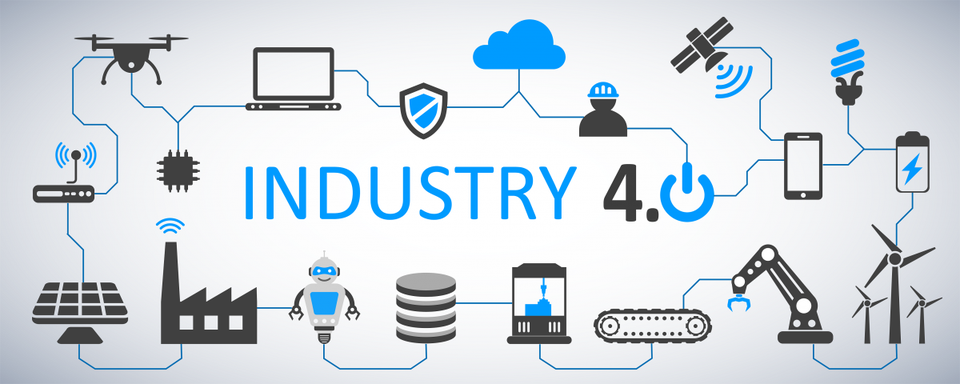
\includegraphics[width=\textwidth]{./chapter-intro/images/intro/forbes-i40.png}
		\label{fig:intro:forbes-i40}
		\caption{Industry 4.0: Incorporating the benefits of machine learning, massive data, mobility, and autonomy within the modern factory.  }
	\end{center}
\end{figure}
%\begin{verbatim}https://www.forbes.com/sites/bernardmarr/2018/09/02/what-is-industry-4-0-heres-a-super-easy-explanation-for-anyone/#6dee527a9788\end{verbatim}

Industry 4.0 is a term used to describe the latest evolution trend in global industrialization with respect to manufacturing.  It is marked by the ambitious end goal of a completely automated and data-driven factory enterprise.  The concept of Industry 4.0 is centered around the smart factory in which . 

Computer

“Industry 4.0” is an abstract and complex term consisting of many components when looking closely into our society and current digital trends. To understand how extensive these components are, here are some contributing digital technologies as examples:[25]

Mobile devices
Internet of Things (IoT) platforms
Location detection technologies
Advanced human-machine interfaces
Authentication and fraud detection
3D printing
Smart sensors
Big data analytics and advanced algorithms
Multilevel customer interaction and customer profiling
Augmented reality/ wearables
Fog, Edge and Cloud computing
Data visualization and triggered "real-time" training
Mainly these technologies can be summarized into four major components, defining the term “Industry 4.0” or “smart factory”:[25]

Cyber-physical systems
IoT
Cloud computing
Cognitive computing

\section{Manufacturing Enterprise}
ISA-95 model of distributed hierarachical: Batch production, Job production, Flow production
Modern paradigms: Edge computing, AI/ML


\begin{figure}[!tbp]
	\begin{center}
		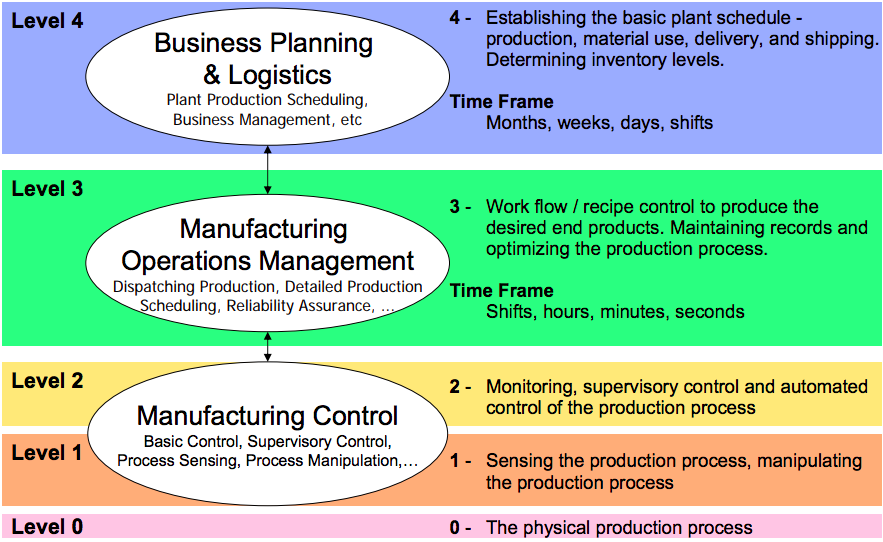
\includegraphics[width=\textwidth]{./chapter-intro/images/intro/isa95-2.png}
		\label{fig:intro:isa95}
		\caption{The ISA-95 model: Legacy enterprise model developed by the ISA which divides production systems into 5 distinct levels based on the Purdue Enterprise Reference Architecture (PERA).}
	\end{center}
\end{figure}

Unlike the MESA model, which focused on business process, the ISA-95 model focuses on information architecture. The ISA-95 model divides production systems into 5 levels, based on the Purdue Enterprise Reference Architecture (PERA) model.

In this way, the ISA-95 standard helps define boundaries between systems. Intelligent devices, such as sensors, belong to Level 1. Control systems such as PLCs , DCS, OCS, belong to Level 2. MES, belong to Level 3. ERP to level 4.

By situating MES on Level 3, ISA-95 implies that MES connect production with enterprise systems, manage workflows to produce end products, maintain records of production, and optimize the production process.

The goal was to develop a standard that would enable efficient interfacing and integration between an ERP system and an MES. This would facilitate effective communication between stakeholders, lowering the total cost of ownership and enabling error-free integration.


\section{The Importance of Wireless in Automation}

The fourth industrial revolution, commonly referred to as Smart Manufacturing in the U.S. and Industry 4.0 in Europe, promises unparalleled productivity and capability advances in the manufacturing.  Propelled by economic pressure toward greater efficiency, factory agility, and product customization, future factories will have the technological ability to adapt to customer demands quickly, modify manufacturing processes automatically based on quality feedback, and fabricate products with a reduced environmental impact.  Technological advances required for smart manufacturing to be truly successful include a collaborative and mobile robotics, distributed machine autonomy based on artificial intelligence, and a high degree of interconnectivity of among the automation resources.  Robots will work together and with people to accomplish complex tasks.  Robots will have the ability to roam between work-cells within a factory, learn its role quickly, become aware of edge devices, and communicate with other actors within the work-cell to accomplish its goals.  Current manufacturing architectures use wired connectivity through field bus and industrialized Ethernet for sensing and real-time control.  

Indeed, through advances in time-sensitive networking, many of the promises of smart manufacturing are being realized; however, the true goals of smart manufacturing require a large deployment of sensing and actuation devices and untethered (i.e. mobile), autonomous robotics actors.  The use of wires precludes mobility and makes deployment of edge devices more expensive as each devices requires power, wires, and conduit for communication. By adopting wireless for both sensing and control of machines within the work-cell, a lower-cost, untethered operation is achievable. once wireless is adopted as the primary mode of communication, questions arise as to the required latency, reliability, and scale of the wireless network especially when the network is used for the control of machines and the assurance of safety. 

Latency is defined as the data time-of-flight between two applications, e.g. when an event is acquired at a sensor to the point it is made available at a programmable logic controller (PLC).  Reliability is defined as the data loss probability between two applications. Scale is defined as the number of stations accessing the wireless network.  The requirements of reliability, latency, and scale directly relate to the complexity and cost of the wireless network; therefore, a rigorous analysis, validated by physics and untainted by market hype, is necessary to define realistic, achievable, and cost effective performance parameters of the wireless network.  In this paper, we investigate the validity of commonly advertised requirements of wireless networks used for industrial control systems whiling providing a validated perspective on those requirements making realization of such networks more achievable using existing technologies.  We begin with a close examination of existing wireless network requirements for factory automation. We follow with an architectural analysis of the future collaborative work-cell. This architectural analysis drives a cyberphysical system simulation to determine limits of reliability, latency, and scale constraints of wireless stations within the work-cell.  We then conclude with recommendations for reliability, latency, and scale constraints that will accommodate most industrial automation applications and are realizable with devices that are based on ubiquitous standards.

\section{Challenges in Industrial Wireless Networks}

\subsection{Avoiding the Hype: Understand the Requirements}
\subsection{Interference}
\subsection{Multi-path Propagation}
\subsection{Reliability}
\subsection{Latency in Time-sensitive Applications}
\subsection{Energy Efficiency Application for Battery-powered Devices }
\subsection{Trading Reliability, Latency, Scale, and Power}

\subsection{Trade-space for Requirements}
Insert special graph showing the competing requirements

\section{Industrial Wireless Use Cases}

\section{Plethora of Wireless Technologies}
Explain the plethora of wireless tech available, difficulty understanding which if any tech is applicable to a particular use case

Show the resilience week paper

Show 

\section{Need for Evaluation Methods }
Explain how testing the communication network is not sufficient.  need to test the impact of network on the physical system.  Need methods by which to do this.  Start with requirements, proceed to design of the system, and then verification of performance of network AND physical system, and then feedback into design/requirements.

Need to show the architecture

L'objectif principal de votre thèse peut être mis en avant à l'aide de l'environnement ci-dessous:

\iftoggle{usingspim}{
	\begin{emphbox}
		Proposer un modèle qui fait quelque chose!
	\end{emphbox}
}

\chapter{Thesis Summary}

\section{Thesis Objectives}

\section{Thesis Organization}

We are going to provide a visual map of how it all fits together: flow chart of activities, papers, and data outputs

